\documentclass{subfiles}

\begin{document}
  \section{Objective}
  Analysis on the 3 epidemic models, SIR, SIS, SIRS. And effect of network structure has upon the epidemic models.
  \section{Methodology}
  \subsection{Data Source}
  A Slashdot dataset is chosen to be the underlying social network of this epidemic simulation. Slashdot is a science and technology related social news website which is famous for its specific user community. In 2002, Slashdot allowed users to tag each other as friends or foes. The network used contains friends/foes links between the users of the Slashdot in Febuary,
  \section{Dataset Statistics}
  The table below shows the data generated using SNAP.py on the dataset Slashdot0922. 2009\cite{leskovec2008community, snapnets}. The dataset is acquired from SNAP Stanford\cite{snapnets}.
  \subsection{Tool}
  Snap.py by the Stanford University was used to simulate the social network. Graph manipulation and social network simulation was done using Snap.py on Windows 10 and Windows Subsystem for Linux\cite{leskovec2016snap}.

  Numpy is used in the program for stating the state of each node in the social network and for after-processing the simulation data\cite{2020SciPy-NMeth}.

  Scikit-learn is used to do linear regression on simulation data of SIS model for prediction in order to replace long computation of equilibrium points of SIS model\cite{scikit-learn}.

  A list of other libraries used for analysis of data is provided below\cite{snapnets}.
  \begin{itemize}
    \item Matplotlib \cite{Hunter:2007}
  \end{itemize}

  \subsection{Experiment Design}
  In this project, the three SIR, SIRS, SIS epidemic models are simulated using SNAP.py on Python 3. Every node in the network is assumed to be a person and every directed edge in the network is assumed to be a contact. Initially, all nodes in the network is assumed susceptible to the epidemic(S). A random number of \(s\) people in the network would be infected(I) by the epidemic. And for each contact, the disease will have \(p\) probability to transmit to the uninfected nodes in each wave(\(t\)). For each infected person, they will be infectious for \(i\) waves. And if they have a temperary immune to the epidemic after infection, the immunity will exist for \(r\) days. The epidemic ends at wave \(t_end\) if there is no infected(I) in network.

  A series of tests will be conducted by changing parameters \(p, r, i, s\) for observation on SIR, SIRS and SIS epidemic models. The observation will be based on average amount of infected(I) and time(\(t\)) needed for the epidemic to end and no nodes in the network are infected.

  As the time(\(t\)) needed for epidemic to end in SIRS and SIS models is large, the amount of iterations of infection waves will be limited to 100 iterations and the termination time of the epidemics will be predicted using regression on peak infected values and the number of infected of each wave.

  The effect of network structure will also be investigated by randomly removing or adding a certain amount of edges to increase and decrease effective diameter of the network and the size of stronly connected components to investigate the effect of network structure in epidemics.

  \section{Dataset Statistics}
  \subsection{Graph Statistics}
  The table below shows statistics of the Slashdot0922 dataset\cite{snapnets} generated using SNAP.py\cite{leskovec2016snap}.

  \begin{tabular}{|l|l|}
    \hline
    Slashdot0922: & Directed\\
    \hline
    Nodes: & 82168\\
    \hline
    Edges: & 948464\\
    \hline
    Zero Degree Nodes: & 0\\
    \hline
    Zero In-degree Nodes: & 0\\
    \hline
    Zero Out-degree Nodes: & 3727\\
    \hline
    Non-zero In-out Degree Nodes: & 78441\\
    \hline
    Unique Directed Edges: & 870161\footnote{smaller value from snap.CntUniqDirEdges() used instead of 948464 from snap.PrintInfo}\\
    \hline
    Unique Undirected Edges: & 504230\footnote{smaller value from snap.CntUniqUndirEdges() used instead of 582533 from snap.PrintInfo()}\\
    \hline
    Unique Bidirectional Edges: & 365931\\
    \hline
    Self Edges: & 78303\\
    \hline
    Zero Out-degree Nodes (Self Edges Removed): & 10277\\
    \hline
    Non-zero In-out Degree Nodes (Self Edges Removed): & 71891\\
    \hline
    Closed Triads/Closed Triangles: & 602592\\
    \hline
    Open Triads/Open Triangles: & 73175813\\
    \hline
    Fraction of Closed Triads: & 0.008168\\
    \hline
    Average Clustering Coefficient: & 0.063449\\
    \hline
    Size of Largest Strongly Connected Component: & 0.86782\\
    \hline
    Weakly Connected: & True\\
    \hline
    Size of Largest Weakly Connected Component: & 1.0\\
    \hline
    90\% Effective Diameter: & 4.688472\footnote{smaller value in snap.PrintInfo() is used}\\
    \hline
    95\% Effective Diameter: & 4.9328\\
    \hline
    Approx. Full Diameter: & 11\\
    \hline
  \end{tabular}

  \subsection{In-degree}
  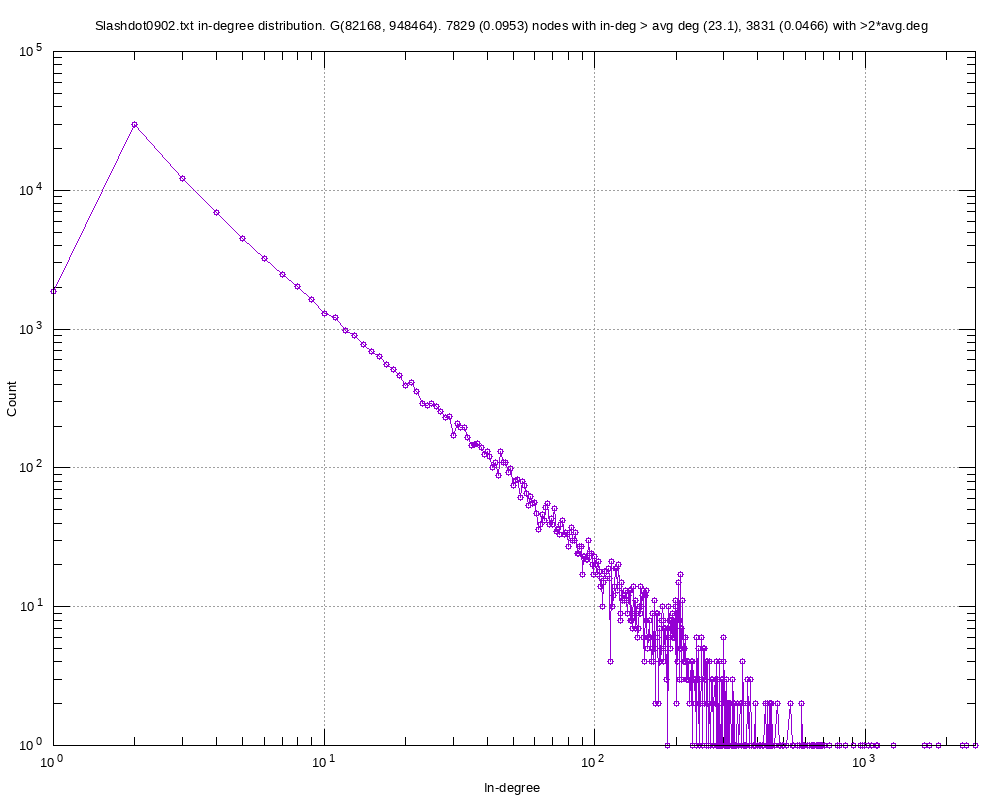
\includegraphics[scale=0.6]{InDegDist.png}\\
  \begin{center}
  \begin{tabular}{|l|l|}
    \hline
    & Number of Edges\\
    \hline
    Max: & 2553\\
    \hline
    Average: & 1.4759\\
    \hline
    Min: & 1\\
    \hline
  \end{tabular}
  \end{center}

  \subsection{Out-degree}
  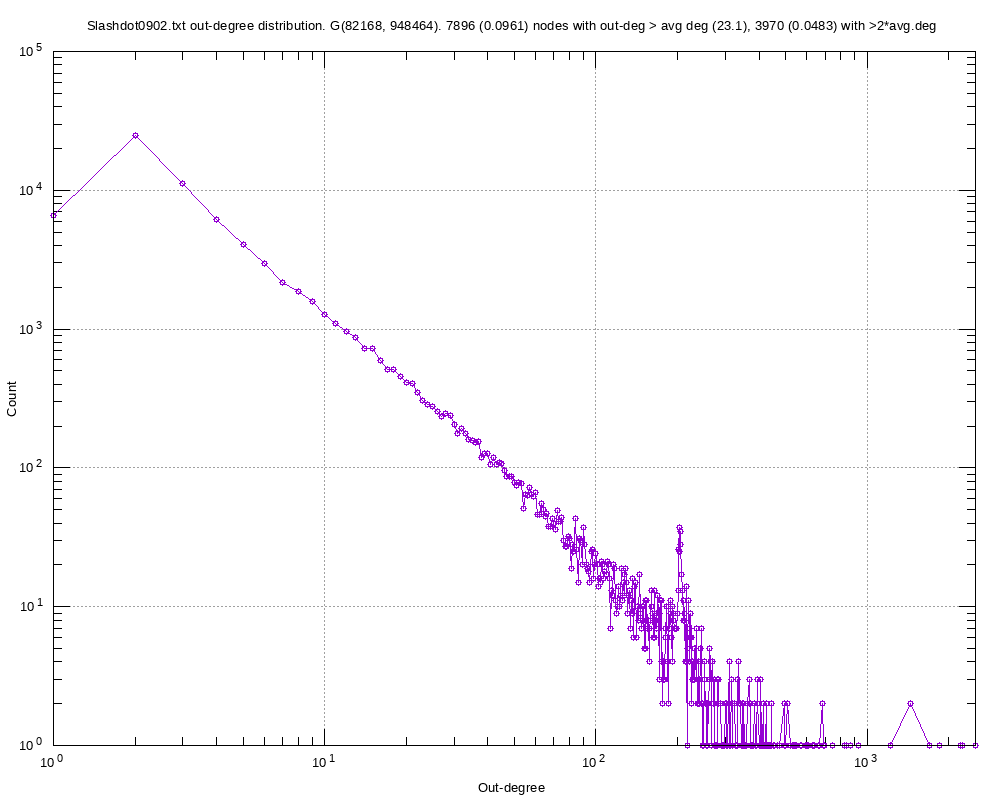
\includegraphics[scale=0.6]{OutDegDist.png}\\
  \begin{center}
  \begin{tabular}{|l|l|}
    \hline
    & Number of Edges\\
    \hline
    Max: & 2511\\
    \hline
    Average: & 1.3189\\
    \hline
    Min: & 0\\
    \hline
  \end{tabular}
  \end{center}

  \subsection{Strongly Connected Components}
  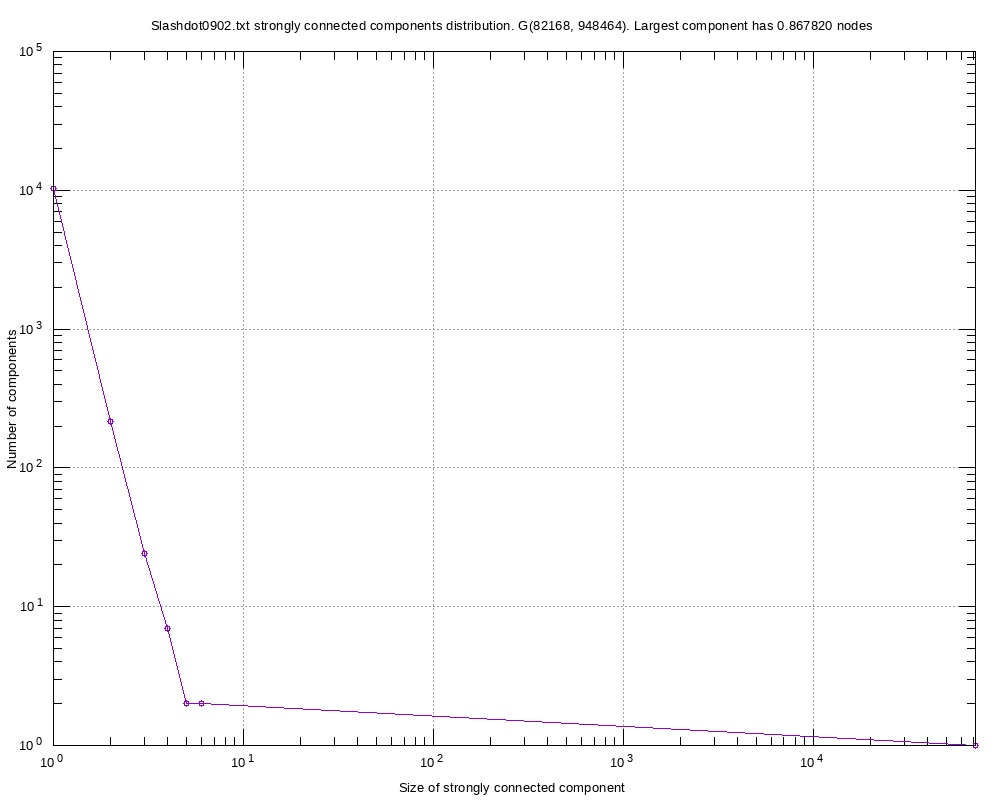
\includegraphics[scale=0.6]{SccDist}

  Given the network is weakly connected, and there is no nodes of zero in and out degrees, all nodes are connected to each other with at least one in or out edge. The small 90\%, 95\% effective diameter and the 0.86782 fraction of nodes in the largest strongly connected component demonstrate a large amount of nodes are interconnected and there is a probability of \(0.86782^2\) that there exists a path from any node in the node in the network to another node in the network. And after removing self edges, there are 0.010835 fraction of nodes have no outgoing edges in the network, implies they are only included in some other nodes' circles, forms sinks in the network but not connect themselves to each other.
\end{document}
